\chapter{Partizioni binarie del piano e RandAuto}

\section{Il problema della partizione binaria del piano}

\scan{60}

Dati $n$ segmenti del piano a due a due \emph{non intersecanti}, vogliamo partizionare il
piano in modo tale che in ogni regione ci sia al più un segmento, oppure una parte di esso.
Scriveremo $S=\set{s_1,\dots,s_n}$ per l'insieme dei segmenti dati, e useremo indifferentemente
$n$ e $\abs{S}$ per la loro cardinalità. Una partizione di questo tipo si chiama
\emph{partizione binaria del piano} (\emph{binary planar partition}, in breve BPP): «binaria»
perché la si costruisce tagliando ripetutamente una regione in due con una retta.

\begin{esempio}
Cinque segmenti $s_1,\dots,s_5$ e una partizione che li separa. I tagli (tratteggiati)
vengono eseguiti uno dopo l'altro, ciascuno all'interno della regione che si vuole spezzare,
e producono le sei regioni $r_1,\dots,r_6$. Uno dei tagli attraversa $s_3$ e lo spezza in due
parti, che finiscono in due regioni diverse ($r_6$ e $r_4$): per questo le regioni sono
\emph{sei} e non cinque.

\begin{figure}[H]
\centering
% Esempio di partizione binaria del piano (BPP) per cinque segmenti non
% intersecanti.  Tratto pieno = segmenti s_1,...,s_5; tratteggio = rette di
% taglio l_1,...,l_5, disegnate nell'ordine in cui la partizione le esegue
% (ogni taglio vive soltanto dentro la regione che spezza, e l_3 termina con
% una giunzione a T su l_2).  L'unico segmento attraversato da un taglio e'
% s_3: lo spezza l_2, e le due porzioni finiscono in r_4 (quella bassa) e in
% r_6 (quella alta).  Sei regioni per cinque segmenti.
%
% Ogni taglio agisce su una regione che contiene almeno due porzioni di
% segmento, come vuole la costruzione:
%   l_1 : {s_5}            | resto
%   l_2 : r_4 = {s_3 basso}| resto
%   l_3 : r_6 = {s_3 alto} | resto
%   l_4 : r_2 = {s_1}      | resto
%   l_5 : r_5 = {s_4}      | r_3 = {s_2}
\begin{tikzpicture}[
    scale=0.95,
    segmento/.style={draw=black,line width=1.3pt,line cap=round},
    taglio/.style={draw=graydark,line width=0.7pt,line cap=round,
                   dash pattern=on 3.2pt off 2.4pt},
    et/.style={font=\footnotesize},
    etg/.style={font=\footnotesize,text=graydark},
  ]

  % ---- riquadro implicito (nessuna cornice disegnata) ---------------------
  \useasboundingbox (-0.15,-0.55) rectangle (9.15,6.05);

  % ---- rette di taglio, nell'ordine di esecuzione -------------------------
  % l_1: taglia tutto il piano
  \draw[taglio] (0,4.10) -- (9,4.10);
  \node[etg] at (0.42,4.36) {$\ell_1$};
  % l_2: taglia il semipiano inferiore e spezza s_3
  \draw[taglio] (1.45,4.10) -- (3.438,0);
  \node[etg] at (3.44,-0.28) {$\ell_2$};
  % l_3: taglia la regione a destra di l_2 (giunzione a T su l_2)
  \draw[taglio] (2.75,4.10) -- (2.4683,2.00);
  \node[etg] at (3.05,3.80) {$\ell_3$};
  % l_4: taglia la regione a destra di l_3
  \draw[taglio] (5.15,4.10) -- (7.60,0);
  \node[etg] at (7.60,-0.28) {$\ell_4$};
  % l_5: taglia la regione compresa fra l_2 e l_4
  \draw[taglio] (2.856,1.20) -- (5.7296,3.13)
        node[etg,pos=0.86,below=2.5pt,sloped] {$\ell_5$};

  % ---- segmenti -----------------------------------------------------------
  \draw[segmento] (2.00,5.30) -- (2.70,4.35);           % s_5, sopra l_1
  \draw[segmento] (1.00,1.60) -- (2.15,2.95);           % s_3, spezzato da l_2
  \draw[segmento] (3.10,2.40) -- (5.00,3.75);           % s_4
  \draw[segmento] (4.60,1.55) -- (4.85,0.85);           % s_2
  \draw[segmento] (6.50,2.60) -- (8.20,2.45);           % s_1

  % punto in cui l_2 spezza s_3
  \filldraw[fill=white,draw=black,line width=0.5pt] (2.059,2.844) circle (1.7pt);

  % ---- etichette dei segmenti --------------------------------------------
  \node[et] at (3.00,4.98) {$s_5$};
  \node[et] at (0.72,2.50) {$s_3$};
  \node[et] at (3.90,2.66) {$s_4$};
  \node[et] at (5.20,1.18) {$s_2$};
  \node[et] at (7.45,2.92) {$s_1$};

  % ---- etichette delle regioni -------------------------------------------
  \node[et] at (7.50,5.20) {$r_1$};   % sopra l_1: contiene s_5
  \node[et] at (2.20,3.55) {$r_6$};   % fra l_2 e l_3, sotto l_1: porzione alta di s_3
  \node[et] at (1.30,1.35) {$r_4$};   % a sinistra di l_2: porzione bassa di s_3
  \node[et] at (2.92,2.10) {$r_5$};   % fra l_3, l_4 e sopra l_5: contiene s_4
  \node[et] at (3.90,0.60) {$r_3$};   % sotto l_5: contiene s_2
  \node[et] at (8.30,0.90) {$r_2$};   % a destra di l_4: contiene s_1
\end{tikzpicture}

\caption{Una partizione binaria del piano per cinque segmenti non intersecanti: in tratto
continuo i segmenti $s_1,\dots,s_5$, tratteggiate le rette di taglio. Ognuna delle sei
regioni $r_1,\dots,r_6$ contiene esattamente un segmento o una porzione di segmento;
$s_3$ è l'unico segmento spezzato.}
\end{figure}
\end{esempio}

\begin{domanda}
Dati $n$ segmenti, esiste sempre una partizione che genera $n$ regioni?
\end{domanda}

La risposta è \emph{no}, ed eppure i segmenti che bastano a farla cadere sono soltanto tre:
tre segmenti disposti «a girandola» — ciascuno rivolto verso il successivo, e a due a due
non intersecanti — non si lasciano separare da sole tre regioni.
Tagliando con la retta che prolunga $s_2$ si spezza $s_3$ in due parti; con altri due tagli,
le rette che prolungano $s_1$ e $s_3$, si isolano i quattro frammenti così ottenuti. Le
regioni finali sono quattro.

\begin{figure}[H]
\centering
% Tre segmenti «a girandola»: nessuna partizione binaria del piano riesce a
% separarli con tre sole regioni.  Tratto pieno = i segmenti; tratteggio = le
% rette che li prolungano, usate come tagli.  Prima si taglia con l(s_2), che
% attraversa s_3 e lo spezza; poi, nel semipiano superiore, con l(s_1) e, in
% quello inferiore, con l(s_3).  Ogni taglio e' disegnato solo dentro la
% regione che spezza, quindi l(s_1) e l(s_3) si fermano su l(s_2).
% Risultato: quattro regioni r_1,...,r_4 per tre segmenti.
\begin{tikzpicture}[
    scale=1.0,
    segmento/.style={draw=black,line width=1.3pt,line cap=round},
    taglio/.style={draw=graydark,line width=0.7pt,line cap=round,
                   dash pattern=on 3.2pt off 2.4pt},
    et/.style={font=\footnotesize},
    etg/.style={font=\footnotesize,text=graydark},
    testo/.style={font=\footnotesize},
  ]

  \useasboundingbox (-0.10,-0.10) rectangle (8.60,5.70);

  % ---- rette di taglio -----------------------------------------------------
  % l(s_2): il primo taglio, attraversa tutto il piano e spezza s_3
  \draw[taglio] (0.30,2.4042) -- (7.30,2.2875);
  \node[etg,anchor=west] at (7.38,2.30) {$\ell(s_2)$};
  % l(s_1): taglia il semipiano superiore, si ferma su l(s_2)
  \draw[taglio] (2.6191,5.30) -- (4.704,2.3311);
  \node[etg] at (2.42,5.48) {$\ell(s_1)$};
  % l(s_3): taglia il semipiano inferiore, si ferma su l(s_2)
  \draw[taglio] (2.3634,0.30) -- (3.5138,2.3506);
  \node[etg,anchor=north east] at (2.30,0.22) {$\ell(s_3)$};

  % ---- i tre segmenti (a due a due non intersecanti) ----------------------
  \draw[segmento] (2.70,0.90) -- (3.85,2.95);   % s_3, spezzato da l(s_2)
  \draw[segmento] (3.05,4.686) -- (4.42,2.735); % s_1
  \draw[segmento] (3.80,2.3459) -- (6.55,2.30);  % s_2, giace su l(s_2); l'estremo
                                                 % sinistro sta staccato dal punto
                                                 % in cui l(s_2) spezza s_3

  % punto in cui l(s_2) spezza s_3
  \filldraw[fill=white,draw=black,line width=0.5pt] (3.5138,2.3506) circle (1.7pt);

  % ---- etichette dei segmenti --------------------------------------------
  \node[et] at (2.80,1.90) {$s_3$};
  \node[et] at (4.34,3.30) {$s_1$};
  \node[et] at (5.00,1.98) {$s_2$};

  % ---- etichette delle regioni -------------------------------------------
  \node[et] at (2.00,3.90) {$r_4$};   % sopra l(s_2), a sinistra di l(s_1): porzione alta di s_3
  \node[et] at (5.60,4.10) {$r_2$};   % sopra l(s_2), a destra di l(s_1): contiene s_1
  \node[et] at (1.80,1.30) {$r_3$};   % sotto l(s_2), a sinistra di l(s_3): porzione bassa di s_3
  \node[et] at (5.10,0.85) {$r_1$};   % sotto l(s_2), a destra di l(s_3): contiene s_2

  % ---- annotazione --------------------------------------------------------
  \node[testo,anchor=west] at (6.55,1.55) {3 segmenti};
  \node[testo,anchor=west] at (6.55,1.05) {4 regioni};
\end{tikzpicture}

\caption{Tre segmenti bastano a impedire una partizione con tre sole regioni. Le tre rette
tratteggiate prolungano i tre segmenti; la prima, quella di $s_2$, spezza $s_3$, e le
regioni finali sono quattro: $r_1,\dots,r_4$.}
\end{figure}

Il numero di regioni, dunque, può eccedere il numero dei segmenti. La domanda interessante
diventa allora \emph{di quanto} lo può eccedere: bastano sempre $\Oh(n)$ regioni? È una
domanda tutt'altro che facile, e per porla in modo preciso conviene prima darsi una
rappresentazione formale delle partizioni.

\section{La BPP come albero binario}

\scan{61}

Rappresenteremo una BPP come un \emph{albero binario} i cui nodi interni sono coppie
\[
  (r,\ \ell)
\]
dove $r$ è la \emph{regione} associata al nodo e $\ell$ è il \emph{limite}, cioè la retta
che divide $r$: i due figli del nodo corrispondono alle due sottoregioni in cui $\ell$ taglia
$r$. Ogni foglia è etichettata dal segmento — o dalla porzione di segmento — contenuto nella
regione corrispondente. Chiamiamo \emph{dimensione} della partizione $P$ il numero delle sue
foglie, e la indichiamo con $\abs{P}$: è la quantità che vogliamo tenere piccola.

Le foglie sono almeno $n$, e possono essere di più.

\begin{esempio}
Sia $S=\set{s_1,s_2,s_3}$. La prima retta $\ell_1$ attraversa $s_3$ e lo spezza nelle due
porzioni $s_{3,1}$ e $s_{3,2}$: da una parte di $\ell_1$ restano $s_1$ e $s_{3,1}$, che
vengono separati da $\ell_2$; dall'altra restano $s_2$ e $s_{3,2}$, separati da $\ell_3$.
L'albero ha allora tre nodi interni e \emph{quattro} foglie, una in più dei tre segmenti di
partenza, proprio perché $s_3$ è stato spezzato.

\begin{figure}[H]
\centering
% Una BPP di S = {s_1,s_2,s_3} e l'albero binario che la rappresenta.
% A sinistra la scena: la prima retta l_1 taglia tutto il piano e attraversa
% s_3, spezzandolo in s_{3,1} (sopra l_1) e s_{3,2} (sotto l_1); l_2 e l_3
% sono i tagli delle due regioni figlie e sono quindi semirette che partono
% da l_1 e non la oltrepassano.
% A destra l'albero: nodi interni = coppie (r,l), foglie = segmenti o porzioni
% di segmento.  Tre nodi interni (tre tagli) e quattro foglie = 3 segmenti + 1
% spezzamento; le due foglie evidenziate sono le due porzioni di s_3.
\begin{tikzpicture}[
    segmento/.style={draw=black,line width=1.3pt,line cap=round},
    taglio/.style={draw=graydark,line width=0.7pt,line cap=round,
                   dash pattern=on 3.2pt off 2.4pt},
    et/.style={font=\footnotesize},
    etg/.style={font=\footnotesize,text=graydark},
    interno/.style={ellipse,draw=black,line width=0.6pt,inner sep=1.5pt,
                    minimum width=1.5cm,minimum height=0.74cm,font=\footnotesize},
    foglia/.style={circle,draw=black,line width=0.6pt,inner sep=0.5pt,
                   minimum size=0.76cm,font=\footnotesize},
    spezzata/.style={foglia,fill=accent!25},
    arco/.style={draw=black,line width=0.6pt},
  ]

  %% ======================= (a) la scena ==================================
  \begin{scope}[scale=0.78]

    % l_1: primo taglio, attraversa tutto il piano e spezza s_3
    \draw[taglio] (0.80,7.05) -- (6.50,2.10);
    \node[etg] at (6.90,1.80) {$\ell_1$};
    % l_2: taglia la regione sopra l_1 (semiretta uscente da l_1)
    \draw[taglio] (4.00,4.271) -- (6.10,6.85);
    \node[etg] at (6.42,7.10) {$\ell_2$};
    % l_3: taglia la regione sotto l_1 (semiretta uscente da l_1)
    \draw[taglio] (3.50,4.705) -- (3.85,1.15);
    \node[etg] at (3.92,0.78) {$\ell_3$};

    % i tre segmenti
    \draw[segmento] (2.30,6.00) -- (4.30,6.80);   % s_1
    \draw[segmento] (1.30,5.85) -- (2.40,3.80);   % s_2
    \draw[segmento] (4.40,3.20) -- (5.80,5.05);   % s_3, spezzato da l_1

    % punto in cui l_1 spezza s_3
    \filldraw[fill=white,draw=black,line width=0.5pt] (4.7305,3.6368) circle (2.2pt);

    \node[et] at (3.00,7.15) {$s_1$};
    \node[et] at (0.95,4.90) {$s_2$};
    \node[et] at (6.10,5.25) {$s_3$};
    \node[etg] at (5.72,4.00) {$s_{3,1}$};
    \node[etg] at (4.30,2.72) {$s_{3,2}$};
  \end{scope}

  %% ======================= (b) l'albero ==================================
  \begin{scope}[shift={(8.60,1.55)}]
    \node[interno] (n1) at ( 0.00,3.00) {$r_1\ \ \ell_1$};
    \node[interno] (n2) at (-1.50,1.50) {$r_2\ \ \ell_2$};
    \node[interno] (n3) at ( 1.50,1.50) {$r_3\ \ \ell_3$};

    \node[foglia]   (f1) at (-2.10,0.00) {$s_1$};
    \node[spezzata] (f2) at (-0.90,0.00) {$s_{3,1}$};
    \node[foglia]   (f3) at ( 0.90,0.00) {$s_2$};
    \node[spezzata] (f4) at ( 2.10,0.00) {$s_{3,2}$};

    \draw[arco] (n1) -- (n2);
    \draw[arco] (n1) -- (n3);
    \draw[arco] (n2) -- (f1);
    \draw[arco] (n2) -- (f2);
    \draw[arco] (n3) -- (f3);
    \draw[arco] (n3) -- (f4);
  \end{scope}
\end{tikzpicture}

\caption{Una BPP di $S=\set{s_1,s_2,s_3}$ (a sinistra la scena, a destra l'albero che la
rappresenta). La retta $\ell_1$ spezza $s_3$ in $s_{3,1}$ e $s_{3,2}$: le foglie sono
quattro, una più dei segmenti.}
\end{figure}
\end{esempio}

\begin{osservazione}
L'albero che rappresenta la $\mathrm{BPP}(S)$ è sempre un albero binario con un numero di
foglie pari a
\[
  \#\text{foglie} \;=\; n + \#\text{tagli},
\]
dove $\#\text{tagli}$ conta i tagli che spezzano un segmento: ogni taglio che spezza un
segmento produce una porzione in più, e quindi una foglia in più (un segmento attraversato da
$k$ tagli dà origine a $k+1$ porzioni). Questo numero non dipende solo da $S$, ma dalle scelte
fatte, cioè dalle rette con cui si decide di partizionare.
\end{osservazione}

\begin{center}
\fbox{\textbf{Goal:} tenere \emph{basso} il numero di tagli.}
\end{center}

\begin{domanda}[problema aperto]
Esiste sempre una $\mathrm{BPP}(S)$ con $\Oh(\abs{S})$ foglie, cioè con $\Oh(\abs{S})$
frammenti di segmento e quindi $\Oh(\abs{S})$ regioni?
\dubbioinl{negli appunti «Problema aperto» è seguito da una parola fra parentesi, di lettura
incerta: forse un nome proprio, «Clark»}
\end{domanda}

Negli appunti il problema è dato per aperto, come in Motwani--Raghavan da cui la domanda è
ripresa. Quello che sappiamo fare è $\Oh(\abs{S}\log\abs{S})$: diamo infatti un algoritmo
randomizzato, \textsc{RandAuto}, che dimostra che esiste sempre una $\mathrm{BPP}(S)$ con
quel numero di foglie.

\section{Applicazione: il \emph{painter's algorithm}}

\scan{62}

Una prima applicazione delle partizioni binarie del piano è il \emph{painter's algorithm}:
si usa l'albero della BPP come struttura dati per disegnare una scena.

Fissata la posizione dell'osservatore, l'albero viene visitato ricorsivamente: in ogni nodo
interno $(r,\ell)$ si disegna per prima la regione figlia che sta dalla parte di $\ell$
\emph{opposta} all'osservatore e poi l'altra. Si ottiene così un ordine di disegno dal più
lontano al più vicino, in cui gli oggetti vicini sovrascrivono quelli lontani e la rimozione
delle superfici nascoste è automatica. Il tempo di disegno è proporzionale a $\abs{P}$, cioè
al numero di foglie dell'albero: da qui l'interesse per partizioni di dimensione piccola.

\begin{figure}[H]
\centering
% p62-painter -- il painter's algorithm sull'albero di una BPP.
%
% La scena e' una regione irregolare del piano che contiene 7 segmenti disgiunti
% (tratto spesso).  Due tagli della BPP (tratteggiati, grigi) la suddividono in
% tre regioni:
%   ell_1  taglia la scena in una parte sinistra e una parte destra;
%   ell_2  parte da un punto interno di ell_1 (pallino grigio) e taglia la sola
%          parte destra in una porzione alta e una bassa.
% L'osservatore sta fuori dalla scena, in basso a sinistra: e' quindi a sinistra
% di ell_1 e sotto ell_2.  La visita ricorsiva dell'albero disegna per prima la
% regione dalla parte di ell opposta all'osservatore, quindi nell'ordine
%   (1) destra-alta, (2) destra-bassa, (3) sinistra,
% cioe' dal piu' lontano al piu' vicino.  I numeri cerchiati nelle regioni e la
% legenda in basso riportano quest'ordine; la gradazione del riempimento va dal
% piu' scuro (disegnato per primo) al piu' chiaro (disegnato per ultimo).
%
% Nota: nel manoscritto i due tagli sono curvi e partono entrambi dallo stesso
% punto del bordo; qui sono rettilinei (i tagli di una BPP sono rette) e ell_2
% nasce nell'interno di ell_1, cosi' da rendere visibile la gerarchia.
\begin{tikzpicture}[
    x=7.30cm, y=7.00cm,
    font=\footnotesize,
    >={Stealth[length=4.2pt,width=3.2pt]},
    bordo/.style={draw=black,line width=0.8pt,line join=round,line cap=round},
    taglio/.style={draw=graydark,line width=0.7pt,line cap=round,
                   dash pattern=on 3.2pt off 2.4pt},
    segmento/.style={draw=black,line width=1.4pt,line cap=round},
    etg/.style={text=graydark,inner sep=1.5pt},
    ordine/.style={circle,draw=graydark,fill=white,line width=0.5pt,
                   inner sep=0pt,minimum size=4.2mm,font=\scriptsize},
    occhio/.style={draw=black,line width=0.8pt},
    raggio/.style={->,draw=black,line width=0.6pt},
    frecciaord/.style={->,draw=graydark,line width=0.5pt},
  ]

  % ---- il bordo della scena (curva chiusa irregolare, schizzo a mano) ------
  \def\scenapath{plot[smooth cycle,tension=0.55] coordinates {
      (0.393,0.941) (0.457,0.927) (0.530,0.929) (0.590,0.948) (0.650,0.979)
      (0.713,0.996) (0.778,0.998) (0.838,0.984) (0.893,0.962) (0.918,0.949)
      (0.905,0.888) (0.893,0.815) (0.888,0.762) (0.910,0.710) (0.948,0.665)
      (0.996,0.626) (1.002,0.559) (0.996,0.488) (0.980,0.431) (0.957,0.357)
      (0.923,0.294) (0.877,0.247) (0.824,0.216) (0.767,0.201) (0.712,0.201)
      (0.666,0.182) (0.622,0.149) (0.575,0.100) (0.535,0.049) (0.471,0.011)
      (0.402,0.000) (0.347,0.008) (0.310,0.035) (0.295,0.078) (0.285,0.120)
      (0.243,0.116) (0.228,0.152) (0.194,0.172) (0.190,0.214) (0.157,0.240)
      (0.156,0.288) (0.124,0.318) (0.116,0.356) (0.085,0.388) (0.062,0.437)
      (0.043,0.457) (0.052,0.487) (0.030,0.532) (0.010,0.588) (0.002,0.645)
      (0.015,0.689) (0.032,0.723) (0.081,0.781) (0.118,0.793) (0.175,0.803)
      (0.246,0.853) (0.310,0.898)}}

  % estremi dei due tagli
  \coordinate (T)  at (0.3930,0.9410);   % ell_1 : bordo superiore
  \coordinate (Bs) at (0.5750,0.1000);   % ell_1 : bordo inferiore
  \coordinate (M)  at (0.4157,0.8360);   % ell_2 : punto interno di ell_1
  \coordinate (R)  at (0.9960,0.6260);   % ell_2 : bordo destro

  % ---- riempimento delle tre regioni (ritaglio scena + semipiani) ---------
  % (3) regione sinistra -- la piu' vicina all'osservatore, disegnata per ultima
  \begin{scope}
    \clip \scenapath;
    \clip (0.2838,1.4456) -- (0.6842,-0.4046) -- (-0.60,-0.4046) -- (-0.60,1.4456) -- cycle;
    \fill[accent!9] (-0.60,-0.50) rectangle (1.80,1.60);
  \end{scope}
  % (1) regione destra-alta -- la piu' lontana, disegnata per prima
  \begin{scope}
    \clip \scenapath;
    \clip (0.2838,1.4456) -- (0.6842,-0.4046) -- (1.80,-0.4046) -- (1.80,1.4456) -- cycle;
    \clip (-0.0485,1.0040) -- (1.4602,0.4580) -- (1.80,1.60) -- (-0.60,1.60) -- cycle;
    \fill[accent!38] (-0.60,-0.50) rectangle (1.80,1.60);
  \end{scope}
  % (2) regione destra-bassa
  \begin{scope}
    \clip \scenapath;
    \clip (0.2838,1.4456) -- (0.6842,-0.4046) -- (1.80,-0.4046) -- (1.80,1.4456) -- cycle;
    \clip (-0.0485,1.0040) -- (1.4602,0.4580) -- (1.80,-0.60) -- (-0.60,-0.60) -- cycle;
    \fill[accent!21] (-0.60,-0.50) rectangle (1.80,1.60);
  \end{scope}

  % ---- il bordo della scena ----------------------------------------------
  \draw[bordo] \scenapath;

  % ---- i due tagli della BPP ---------------------------------------------
  \draw[taglio] (T) -- (Bs);
  \draw[taglio] (M) -- (R);
  \fill[graydark] (M) circle (1.2pt);
  \node[etg,anchor=south east] at (0.352,0.960) {$\ell_1$};
  \node[etg,anchor=west]       at (1.012,0.646) {$\ell_2$};

  % ---- i sette segmenti della scena --------------------------------------
  \draw[segmento] (0.232,0.574) -- (0.356,0.662);
  \draw[segmento] (0.138,0.453) -- (0.219,0.395);
  \draw[segmento] (0.358,0.421) -- (0.416,0.540);
  \draw[segmento] (0.453,0.283) -- (0.501,0.212);
  \draw[segmento] (0.645,0.853) -- (0.828,0.779);
  \draw[segmento] (0.556,0.376) -- (0.727,0.580);
  \draw[segmento] (0.794,0.462) -- (0.915,0.431);

  % ---- ordine di disegno delle tre regioni -------------------------------
  \node[ordine] at (0.750,0.910) {1};
  \node[ordine] at (0.820,0.335) {2};
  \node[ordine] at (0.140,0.660) {3};

  % ---- l'osservatore ------------------------------------------------------
  \begin{scope}[shift={(-0.250,0.050)}]
    % occhio stilizzato: due archi che formano una lente, con la pupilla
    \draw[occhio] (-4.6mm,0mm) .. controls (-2.4mm, 3.5mm) and ( 2.4mm, 3.5mm)
               .. ( 4.6mm,0mm) .. controls ( 2.4mm,-3.5mm) and (-2.4mm,-3.5mm)
               .. cycle;
    \fill[black] (0mm,0mm) circle (1.15mm);
    % le tre direzioni di vista, a ventaglio verso la scena
    \draw[raggio] (55:6.4mm) -- (55:21mm);
    \draw[raggio] (33:6.4mm) -- (33:21mm);
    \draw[raggio] (14:6.4mm) -- (14:21mm);
  \end{scope}
  \node[anchor=north,yshift=-5.0mm] at (-0.250,0.050) {osservatore};

  % ---- legenda ------------------------------------------------------------
  \node[anchor=east] at (0.452,-0.092) {ordine di disegno:};
  \node[ordine] (o1) at (0.520,-0.092) {1};
  \node[ordine] (o2) at (0.630,-0.092) {2};
  \node[ordine] (o3) at (0.740,-0.092) {3};
  \draw[frecciaord] (o1) -- (o2);
  \draw[frecciaord] (o2) -- (o3);

\end{tikzpicture}

\caption{La scena, con i suoi segmenti, e l'osservatore. I tagli della BPP suddividono la
scena in regioni; l'albero della partizione fornisce, per ogni posizione dell'osservatore,
un ordine di disegno dal più lontano al più vicino.}
\end{figure}

\section{Autopartizioni e l'algoritmo \textsc{RandAuto}}

\begin{definizione}[autopartizione]\label{def:autopartizione}
Un'\emph{autopartizione} è una BPP tale che ogni retta $\ell_i$ che compare nei suoi nodi
interni $(r_i,\ell_i)$ è una delle rette su cui giace un segmento di $S$, o una parte di esso.
\end{definizione}

Per $s\in S$ scriviamo $\ell(s)$ per la retta su cui giace $s$, cioè il prolungamento di $s$
a tutta la retta.

\begin{figure}[H]
\centering
% p62-autopartizione -- il segmento s giace sulla retta ell = ell(s).
% La retta ell (tratteggiata) e' il prolungamento di s (tratto spesso, con le
% crocette agli estremi).  Tagliando la regione corrente con ell si ottengono
% le due regioni r_ell e r'_ell: s sta esattamente sulla loro frontiera comune
% e va assegnato all'una oppure all'altra.  Le due frecce, perpendicolari a
% ell e uscenti dall'estremo superiore di s, indicano proprio questa scelta.
\begin{tikzpicture}[
    font=\footnotesize,
    >={Stealth[length=4pt,width=3pt]},
    retta/.style={line width=0.5pt,dash pattern=on 2.2pt off 2.4pt},
    segmento/.style={line width=1.4pt},
    freccia/.style={->,line width=0.6pt},
  ]

  % ---- la retta ell : direzione (6.5,2.9), cioe' circa 24 gradi -----------
  \coordinate (P0) at (0,0.15);      % estremo sinistro del tratteggio
  \coordinate (P1) at (6.5,3.05);    % estremo destro del tratteggio
  \coordinate (A)  at (2.145,1.107); % estremo inferiore di s   (t = 0.33)
  \coordinate (B)  at (4.290,2.064); % estremo superiore di s   (t = 0.66)

  \draw[retta] (P0) -- (P1);
  \node[inner sep=1pt] at (6.78,3.16) {$\ell$};

  % ---- il segmento s -----------------------------------------------------
  \draw[segmento] (A) -- (B);
  \foreach \P in {A,B}{%
    \draw[line width=0.6pt] ($(\P)+(-1.1mm,-1.1mm)$) -- ($(\P)+(1.1mm,1.1mm)$);
    \draw[line width=0.6pt] ($(\P)+(-1.1mm, 1.1mm)$) -- ($(\P)+(1.1mm,-1.1mm)$);
  }
  \node[inner sep=1pt] at (3.05,1.99) {$s$};

  % ---- le due direzioni possibili, perpendicolari a ell ------------------
  % normale unitaria a ell:  n = (-0.4074, 0.9130)
  \draw[freccia] (4.209,2.247) -- (3.923,2.886);   % verso la regione r_ell
  \draw[freccia] (4.372,1.881) -- (4.657,1.242);   % verso la regione r'_ell

  % ---- le due regioni ----------------------------------------------------
  \node[inner sep=1pt] at (2.05,2.45) {$r_\ell$};
  \node[inner sep=1pt] at (4.95,1.08) {$r'_\ell$};

\end{tikzpicture}

\caption{Il segmento $s$ giace sulla retta $\ell=\ell(s)$: tagliando con $\ell$, $s$ finisce
sulla frontiera comune alle due regioni $r_\ell$ e $r'_\ell$ e va assegnato all'una oppure
all'altra.}
\end{figure}

\begin{osservazione}\label{oss:frontiera}
Definita la retta $\ell$ su cui giace $s$, il segmento $s$ si trova esattamente sulla
frontiera comune alle due regioni in cui $\ell$ divide la regione corrente. Sceglieremo
allora di collocare $s$ nella regione a destra oppure in quella a sinistra, a seconda di
dove conviene: per esempio nella regione con meno porzioni di segmenti. In particolare
$\ell(s)$ non taglia mai $s$, e quindi in un'autopartizione un segmento può essere spezzato
soltanto dalle rette \emph{degli altri} segmenti.
\end{osservazione}

L'algoritmo randomizzato che costruisce un'autopartizione è il seguente.

\begin{algorithm}[H]
\caption{\textsc{RandAuto}}
\begin{algorithmic}[1]
\Require $S=\set{s_1,\dots,s_n}$, segmenti a due a due non intersecanti.
\Ensure $P_\pi$, un'autopartizione binaria del piano (\emph{binary planar autopartition})
di $S$.
\State scegli uniformemente a caso una permutazione $\pi$ di $\set{1,\dots,n}$;
\While{esiste una regione $r$ che contiene più di una porzione di segmento}
    \State taglia $r$ usando $\ell(s_i)$, dove $s_i$ è il primo segmento nell'ordine dato
    da $\pi$ tale che $s_i$ (o una sua porzione) sia contenuto in $r$.
\EndWhile
\end{algorithmic}
\end{algorithm}

Tutte le scelte casuali sono concentrate nel passo~1: una volta estratta $\pi$, il resto
dell'esecuzione è completamente deterministico, e per questo la partizione prodotta si indica
con $P_\pi$.

\section{Analisi: la dimensione attesa di \texorpdfstring{$P_\pi$}{P pi}}

\scan{63}

\begin{teorema}[dimensione attesa di \textsc{RandAuto}]\label{thm:randauto-size}
Il valore atteso della dimensione dell'autopartizione prodotta da \textsc{RandAuto} su un
insieme $S$ di segmenti a due a due non intersecanti è
\[
  \E\bigl[\abs{P_\pi}\bigr]\;=\;\Oh\bigl(\abs{S}\log\abs{S}\bigr),
\]
dove la media è presa sulla scelta uniforme della permutazione $\pi$.
\end{teorema}

Il teorema riguarda la \emph{dimensione dell'output}, non il tempo di esecuzione.

\begin{esercizio}
Dimostrare che il \emph{tempo} di esecuzione di \textsc{RandAuto} su $S$ è, anch'esso in
valore atteso, $\Oh(n^2\log n)$, posto $n=\abs{S}$.
\end{esercizio}

\begin{corollario}[metodo probabilistico]\label{cor:esiste-autopartizione}
Dato $S$, esiste \emph{sempre} una BPP di $S$ di dimensione $\Oh(\abs{S}\log\abs{S})$.
\end{corollario}

\begin{dimostrazione}[del corollario]
Per il teorema esiste una costante $c$ tale che $\E[\abs{P_\pi}]\le c\,n\log n$, con
$n=\abs{S}$. Una variabile aleatoria non può assumere ovunque valori strettamente maggiori
della propria media: esiste quindi almeno una permutazione $\pi_0$ di $\set{1,\dots,n}$ con
$\abs{P_{\pi_0}}\le c\,n\log n$. La partizione $P_{\pi_0}$ è la BPP cercata (anzi, è
addirittura un'autopartizione). Si noti che l'argomento è puramente esistenziale: non
fornisce alcun modo di \emph{esibire} $\pi_0$.
\end{dimostrazione}

\bigskip
\textbf{Dimostrazione del Teorema~\ref{thm:randauto-size}.}
L'\emph{intuizione} è la seguente: dobbiamo stimare quanti tagli di segmenti vengono eseguiti
in un generico \emph{run} dell'algoritmo. Servono due nozioni preliminari.

\begin{definizione}[$\mathrm{index}$]\label{def:index}
Dati $u,v\in S$, definiamo
\begin{align*}
  \mathrm{index}(u,v)&=i
    &&\text{sse } \ell(u) \text{ interseca } i-1 \text{ segmenti prima di intersecare } v,\\
  \mathrm{index}(u,v)&=\infty
    &&\text{sse } \ell(u) \text{ non interseca } v.
\end{align*}
Il conteggio va inteso percorrendo $\ell(u)$ a partire da $u$ nella direzione di $v$; dunque
$\mathrm{index}(u,v)=1$ significa che $v$ è il primo segmento che $\ell(u)$ incontra uscendo
da $u$.
\end{definizione}

\begin{figure}[H]
\centering
% randauto-index -- la definizione di index(u,v) = i.
% Il tratto spesso a sinistra e' il segmento u (con i trattini agli estremi);
% il tratteggio che lo prolunga e' la retta ell(u).  Percorrendo ell(u) a
% partire da u si incontrano i segmenti u_1, u_2, ..., u_{i-1} -- contati
% dalla graffa, i-1 in tutto -- e solo dopo si incontra v.
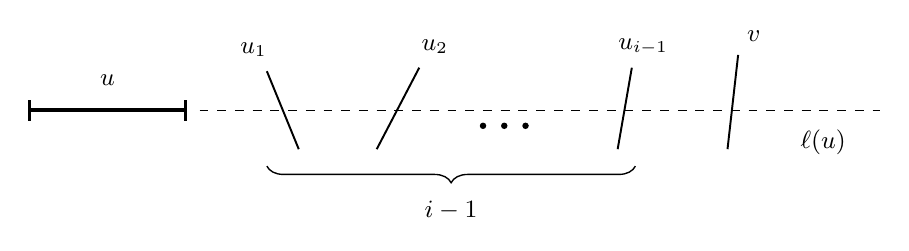
\begin{tikzpicture}[
    scale=0.9,
    font=\small,
    retta/.style={line width=0.5pt,dash pattern=on 3.2pt off 3.2pt},
    segU/.style={line width=1.3pt},
    taglia/.style={line width=0.7pt},
  ]

  % ---- il segmento u e la retta ell(u) -----------------------------------
  \draw[segU] (0,0) -- (2.2,0);
  \draw[segU] (0,-0.15) -- (0,0.15);
  \draw[segU] (2.2,-0.15) -- (2.2,0.15);
  \draw[retta] (2.4,0) -- (12,0);

  \node[inner sep=1pt] at (1.1,0.42) {$u$};
  \node[inner sep=1pt] at (11.2,-0.45) {$\ell(u)$};

  % ---- i segmenti attraversati da ell(u) ---------------------------------
  \draw[taglia] (3.35,0.55) -- (3.80,-0.55);
  \node[inner sep=1pt] at (3.16,0.86) {$u_1$};

  \draw[taglia] (4.90,-0.55) -- (5.50,0.60);
  \node[inner sep=1pt] at (5.72,0.90) {$u_2$};

  \foreach \x in {6.4,6.7,7.0}{\fill (\x,-0.22) circle (1.3pt);}

  \draw[taglia] (8.30,-0.55) -- (8.50,0.60);
  \node[inner sep=1pt] at (8.66,0.90) {$u_{i-1}$};

  \draw[taglia] (9.85,-0.55) -- (10.00,0.78);
  \node[inner sep=1pt] at (10.22,1.05) {$v$};

  % ---- la graffa che conta gli i-1 segmenti intermedi (v escluso) --------
  \draw[line width=0.5pt,decorate,
        decoration={brace,amplitude=6pt,mirror,raise=1pt}]
       (3.35,-0.75) -- (8.55,-0.75);
  \node[inner sep=1pt] at (5.95,-1.42) {$i-1$};

\end{tikzpicture}

\caption{$\mathrm{index}(u,v)=i$: percorrendo $\ell(u)$ a partire da $u$ si incontrano i
segmenti $u_1,u_2,\dots,u_{i-1}$ ($i-1$ in tutto) prima di incontrare $v$.}
\label{fig:randauto-index}
\end{figure}

\begin{definizione}[notazione $u\dashv v$]\label{def:dashv}
Scriviamo
\[
  u\dashv v
\]
se $\ell(u)$ taglia $v$ durante l'esecuzione di \textsc{RandAuto}. È l'evento che corrisponde
all'aggiunta di una porzione di segmento in $P_\pi$.
\end{definizione}

\begin{osservazione}\label{oss:primo-in-pi}
Sia $\mathrm{index}(u,v)=i$ e siano $u_1,\dots,u_{i-1}$ i segmenti che $\ell(u)$ interseca
prima di $v$. Allora $u\dashv v$ si verifica \emph{solo se} $u$ occorre in $\pi$ prima di
$u_1,\dots,u_{i-1},v$. Se infatti uno degli $u_j$ venisse scelto prima di $u$, la retta
$\ell(u_j)$ attraverserebbe il tratto di $\ell(u)$ compreso fra $u$ e $v$, separandoli in due
regioni distinte, e $\ell(u)$ non potrebbe più tagliare $v$; se invece fosse $v$ a precedere
$u$, allora $\ell(v)$ verrebbe usata come taglio prima di $\ell(u)$ e $v$ si troverebbe sulla
frontiera della propria regione (Osservazione~\ref{oss:frontiera}), dove $\ell(u)$ non può
più spezzarlo.

Poiché $\pi$ è scelta uniformemente fra le $n!$ permutazioni, ciascuno degli $i+1$ segmenti
di $\set{u,u_1,\dots,u_{i-1},v}$ ha la stessa probabilità di precedere tutti gli altri. Che
$u$ sia il primo è dunque un evento di probabilità esattamente $\dfrac{1}{i+1}$.
\end{osservazione}

\scan{64}

Introduciamo, per ogni coppia di segmenti distinti $u,v\in S$, la \emph{variabile indicatrice}
dell'evento $u\dashv v$:
\[
  C_{u,v}\;\defeq\;\indic{u\dashv v}\;=\;
  \begin{cases}
    1 & \text{se }\ell(u)\text{ taglia }v\text{ durante l'esecuzione di \textsc{RandAuto}},\\[2pt]
    0 & \text{altrimenti.}
  \end{cases}
\]

Dall'Osservazione~\ref{oss:primo-in-pi} segue immediatamente
\[
  \E\bigl[C_{u,v}\bigr]\;=\;\Pr\bigl[u\dashv v\bigr]\;\le\;\frac{1}{\mathrm{index}(u,v)+1}.
\]
Si noti che la condizione dell'osservazione è soltanto necessaria: per questo si ottiene una
disuguaglianza e non un'uguaglianza.

\begin{osservazione}
Se $\mathrm{index}(u,v)=\infty$, cioè se $\ell(u)$ non interseca affatto $v$, il membro destro
va letto come $0$: in tal caso l'evento $u\dashv v$ è impossibile e $C_{u,v}=0$ con certezza.
\end{osservazione}

\paragraph{Dimensione attesa di $P_\pi$.}
La partizione parte dagli $n=\abs{S}$ segmenti e ogni taglio \emph{effettivo} spezza un
segmento in due, aggiungendo esattamente un frammento (e quindi una foglia occupata). Perciò
la dimensione attesa di $P_\pi$ è $n$ più il numero atteso di tagli:
\begin{align*}
  \E\bigl[\abs{P_\pi}\bigr]
    &\;=\; n+\E\Bigl[\;\sum_{u\in S}\;\sum_{v\in S,\;v\neq u} C_{u,v}\Bigr]\\[2pt]
    &\;=\; n+\sum_{u\in S}\;\sum_{v\neq u}\E\bigl[C_{u,v}\bigr]\\[2pt]
    &\;=\; n+\sum_{u\in S}\;\sum_{v\neq u}\Pr\bigl[u\dashv v\bigr]\\[2pt]
    &\;\le\; n+\sum_{u\in S}\;\sum_{v\neq u}\frac{1}{\mathrm{index}(u,v)+1}.
\end{align*}
Il secondo passaggio è la sola \emph{linearità del valore atteso}: le $C_{u,v}$ non sono
affatto indipendenti, ma qui l'indipendenza non serve.

\begin{osservazione}
Fissato $u$, ci sono \textbf{al più due} segmenti $v$ tali che $\mathrm{index}(u,v)=i$: uno a
destra e uno a sinistra di $u$ lungo $\ell(u)$. Infatti percorrendo $\ell(u)$ a partire da $u$
le direzioni possibili sono solo due e, in ciascuna di esse, il segmento preceduto da
esattamente $i-1$ segmenti è unico.
\end{osservazione}

Raggruppando allora gli addendi della somma interna secondo il valore $i=\mathrm{index}(u,v)$,
che varia fra $1$ e $n-1$ (gli altri segmenti sono $n-1$), si ottiene, per ogni $u\in S$
fissato,
\[
  \sum_{v\neq u}\frac{1}{\mathrm{index}(u,v)+1}\;\le\;\sum_{i=1}^{n-1}\frac{2}{i+1}.
\]

Sostituendo nella stima precedente:
\begin{align*}
  \E\bigl[\abs{P_\pi}\bigr]
    &\;\le\; n+\sum_{u\in S}\;\sum_{i=1}^{n-1}\frac{2}{i+1}
     \;=\; n+2n\sum_{i=1}^{n-1}\frac{1}{i+1}
     \;=\; n+2n\bigl(H_n-1\bigr)\\[2pt]
    &\;\le\; n+2n\,H_n\;\in\;\Oh(n\log n),
\end{align*}
dove $H_n=\sum_{k=1}^{n}\frac{1}{k}=\ln n+\Th(1)$ è l'$n$-esimo numero armonico.

Questo è esattamente l'enunciato del teorema: il valore atteso della dimensione
dell'autopartizione prodotta da \textsc{RandAuto} su un insieme $S$ di $n$ segmenti a due a
due non intersecanti è $\Oh(n\log n)$.
\hfill$\square$

\begin{osservazione}
Il risultato è di Paterson e Yao, e il fattore logaritmico non è un artefatto dell'analisi:
si sa che esistono insiemi di $n$ segmenti in cui \emph{ogni} autopartizione ha
$\Om(n\log n/\log\log n)$ foglie, e dunque per questa via non si arriva a $\Oh(n)$.
\end{osservazione}
